\section{Method}

BID is trained by imitation learning, which we formalized as follows.
Expert demonstrator (drivers) produce an action $a_i$ (ego-vehicle maneuver) when encountering an observation $O_i$, (sensor data, signals) given the expert policy $\pi^{ \star } (O_i)$ (driving skills, attitude, etc.).
The basic idea behind imitation is to train an agent (here BID) that mimics an expert by using these observation.


Prior to training an agent, we need to collect a dataset comprised of observation/action pairs $P= \{ (o_i, a_i) \}_{i=1} ^N $ generated by the expert.
This dataset is in turn used to train a policy $\pi_\theta (o_i)$ which approximateds the expert policy.
The general imitation learning objective is the 
\begin{equation}
	argmin E_{(o_i, a_i) ~ P} [P(\pi_\theta (o_i), a_i )].
\end{equation}

\begin{figure*}[t]
	\centering
	%\fbox{\rule{0pt}{2in} \rule{0.9\linewidth}{0pt}}
	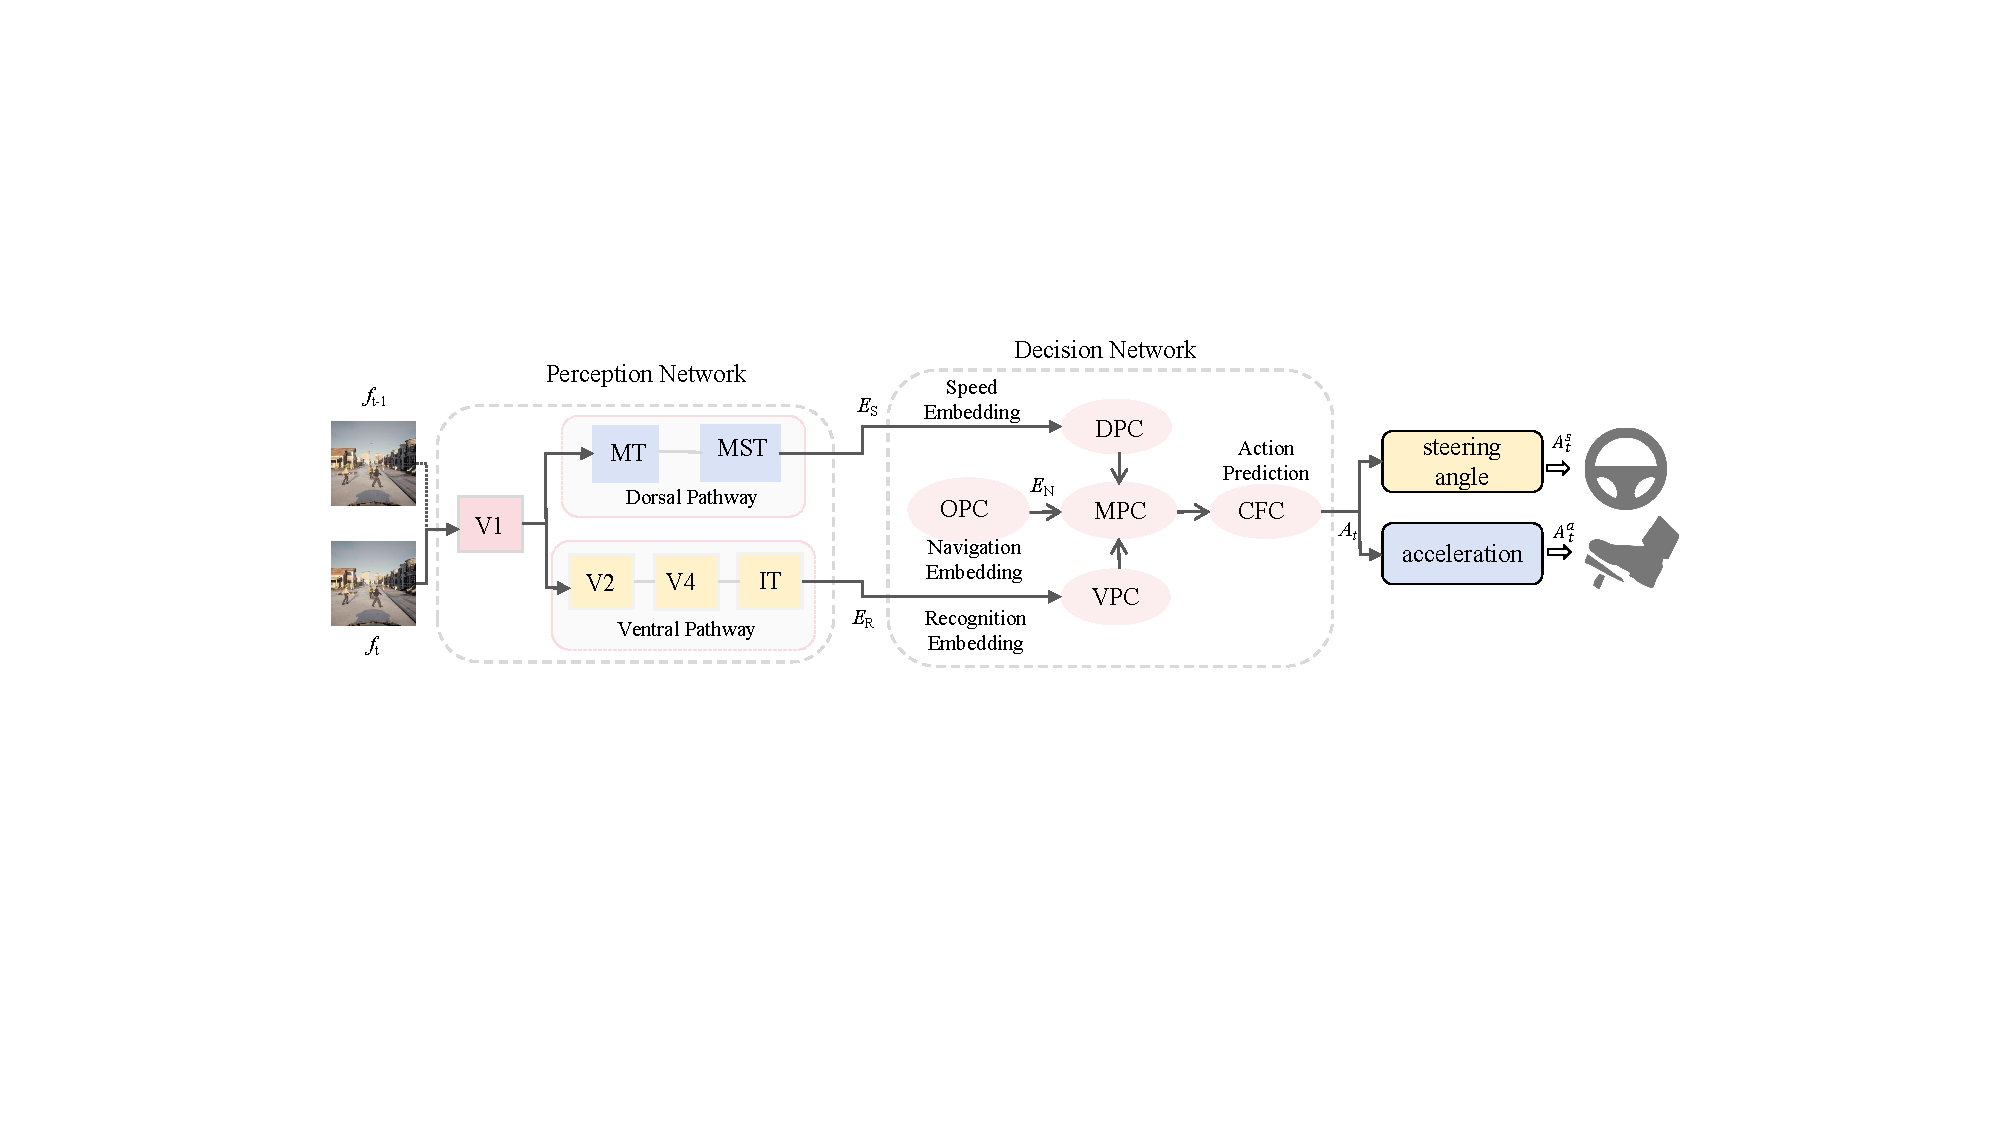
\includegraphics[width=\linewidth]{fig/net}
	\caption{Network architecture of the BID agent:
	our model is mainly comprised of two parts: perception and decision network.
	Perception network include dorsal and ventral pathway to understand their surroundings.
	Decision network include five modules: medial prefrontal cortex (VPC), orbital prefrontal cortex (OPC), caudal prefrontal crotex (CPC), dorsal prefrontal cortex (DPC), ventral prefrontal cortex (VPC).
	Specifically, the input observation consists of RGB image $X_t$.
	The output is action $a_t$, which is directly applied to maneuver to ego-vehicle.
	Since $a_t$ consists of the ego-vehicle's steering angle and acceleration, BID is a vision-based vision-based pure end-to-end AD model.
	Note that these action components are automatically read and associated with the captured images during data collection.
	}
	\label{fig:fig2}
\end{figure*}
\subsection{Neural Aligned Roach}
\hspace{1pc}Drawing inspiration from the brain's exceptional mechanisms in perception and decision-making, we have seamlessly integrated the intricate methods of information processing by brain neurons into an autonomous driving system, aiming to significantly enhance the system's interpretability and robustness. As depicted in Fig. \ref{fig:fig2}, our brain-inspired perception network initially captures precise input data from the surrounding environment, encompassing crucial traffic elements such as roads, vehicles, pedestrians, and traffic signals. Subsequently, this data undergoes meticulous processing through a series of deep convolutional neural networks and recurrent networks, along with the utilization of deep neural network activation functions. This processing mimics the handling of external information by various pathways in the brain's visual cortex. Initially, the primary visual cortex (V1) performs initial processing of visual information, extracting salient features. These features are then relayed to the dorsal visual pathway, where the MT/MST (Middle Temporal and Middle Superior Temporal Areas) encode motion features, specializing in the processing of information related to spatial location and movement. Concurrently, the ventral pathway receives these features, and the IT (Inferior Temporal Cortex) encodes target category information, facilitating object recognition. After this series of processing, our network is able to effectively extract and output multi-dimensional features of the current environment, including the appearance features of objects, motion trajectory features, and the fusion of multi-modal information.

These features are then efficiently transmitted to a brain-inspired decision-making network, undergoing further processing through convolutional and recurrent networks, as well as optimization via deep neural network activation functions. This simulates the processing of sensory outcomes by various regions of the prefrontal cortex in the brain. Among them, the OFC (Orbitofrontal Cortex) plays a vital role in setting future action goals, assisting us in clarifying and locking onto the desired objectives. The MPC ( Medial Prefrontal Cortex) plays a crucial role in making choices based on prior behavioral outcomes, ensuring that our behavior is optimized based on experience. The DPC (Dorsal Prefrontal Cortex) excels at generating goals based on sequences, temporal and spatial environments, providing clear directions and guidance for our actions. The VPC (Ventral Prefrontal Cortex) generates goals based on visual and auditory cues, enabling us to respond quickly and adapt to changes in the external environment.  Meanwhile, the CPC (Caudal Prefrontal Cortex) plays an indispensable role in searching, identifying, or locating specific targets, ensuring that we can accurately locate and focus on the targets.  These regions collaborate and participate in decision-making, generating a highly integrated latent feature vector that precisely encapsulates the critical information required for decision-making. Finally, this latent feature vector is mapped through a carefully designed hidden layer, outputting precise and reliable decision-making information such as driving actions, value function estimates, and speed control.

\textbf{\textsf{Reward Function.}} The BID network aims to mimic the superior information processing capabilities of the human brain by meticulously comparing brain activation patterns with network activation patterns. 
It iteratively updates its network parameters to align network decisions more closely with the actual decision-making mechanisms of the human brain, thereby enhancing the performance and accuracy of the network. 
The specific methodology for updating the network is outlined as follows:
\begin{align}
	\theta_{k+1} & = \arg \max _{\theta} \underset{\tau \sim \pi_{\theta_{k}}}{\mathrm{E}}\left[\mathcal{L}_{\mathrm{ppo}}+\mathcal{L}_{\text {pre }}+\lambda_{\text {e }} \cdot \mathcal{L}_{\text {exp }}\right]
\end{align}

Simulating the approach the brain acquires rewards, aiming to maximize reward-seeking behavior. We train the decision network using Proximal Policy Optimization (PPO) \cite{schulman2017proximal} with clipping. $\mathcal{L}_{\text {ppo }}$ serves as the dopamine reward signal. It is understood that when the brain predicts an upcoming reward, the dopamine system becomes active, generating a reward signal. This signal can be seen as feedback from the brain regarding specific behaviors or situations, informing the brain whether the behavior or situation is positive or worth pursuing. $\mathcal{L}_{\text {pre }}$ represents the prediction error of brain reward. This error arises when there is a deviation between the actual reward and the expected reward. In this context, the reward prediction error functions as a penalty term. Specifically, if the actual reward ($a_{r}$) falls below the expected reward ($p_{r}$), the reward prediction error is negative.Additionally, $\mathcal{L}_{\text {exp }}$ encapsulates the exploration of new actions or strategies during the learning process to obtain more rewards, with $\lambda$ serving as their weight parameter.

Considering both the certainty of the policy (via the entropy regularization term) and the accuracy of reward prediction (via the reward prediction error term), this guides the model to learn more accurate reward predictions, thereby enhancing its performance in reinforcement learning tasks. Specifically, The constant (C) serves to adjust the numerical range or optimization scale of the entropy.
\begin{align}
	\mathcal{L}_{\text{pre}} & = -\lambda_{\text {p }} \cdot [\mathrm{H}\left(\pi_{\theta}\left(\cdot \mid \mathbf{i}_{\mathrm{NR}}, \mathbf{m}_{\mathrm{NR}}\right)\right) - (a_{r} - p_{r})^{2}]
\end{align}
\begin{align}
	\mathrm{H}\left(\pi_{\theta}\right) & = -\mathrm{KL}\left(\pi_{\theta} \| \mathcal{U}(-1,1)\right)+C
\end{align}

Regularizing the whole trajectory to better utilize previous experience and improve the efficiency and stability of learning.
\begin{align}
    \mathcal{L}_{\text {exp }}=\sum_{k=1}^{T} f(k) \cdot \mathrm{KL}\left(\pi_{\theta}\left(\cdot \mid \mathbf{i}_{\mathrm{NR}, k}, \mathbf{m}_{\mathrm{NR}, k}\right) \| p_{z}\right)
\end{align}

\textbf{\textsf{Training.}} The vehicle solely utilizes a single camera sensor to capture raw data of its surrounding environment. At the input stage, it receives a Bird's Eye View (BEV) semantic segmentation image, denoted as $\mathbf{i}_{\mathrm{NR}}$, along with a measurement vector, $\mathbf{m}_{\mathrm{NR}}$, from its own roach system. After acquiring these input data, the BID network is activated to simulate the brain's visual processing. When predicting or receiving rewards, simulated dopamine neurons are activated, releasing dopamine to strengthen memories and behaviors associated with the rewards, increasing the likelihood of repeating these behaviors. During the learning process, there is often a mismatch between expected and actual rewards. When actual rewards exceed expectations, a positive prediction error occurs, further promoting the release of dopamine and thus enhancing the associated behaviors. Through ongoing interaction with the environment, the brain-inspired network adapts behavioral policies by modifying parameters through backpropagation, striving to maximize future rewards.

Multiple driving actions are generated and evaluated separately to assign them respective scores. The driving action with the highest score is then selected to control the movement of the target vehicle.
%\begin{align}
%	S & = r_{1} \mu+r_{2} \lambda
%\end{align}
\subsection{Brain-Expert Mimetic Entity}
\hspace{1pc}\textbf{\textsf{Agent.}} The BID agent utilizes imitation learning to predict driving behavior based on the current state, supervised by extensive data generated by the reinforcement learning expert. The structure of the agent is illustrated in Fig. \ref{fig:fig2}.

\textbf{\textsf{Loss Function.}} In the decision-making stage, for each command, a branch is constructed. All branches share the same architecture, with each branch containing an action head for predicting the continuous action $\mathbf{a}$ and a velocity head for predicting the current vehicle speed $\mathbf{s}$. And $\mathbf{\hat{a}}$ represents the expert's action,$\mathbf{\hat{s}}$ is the measured speed, and $\mathbf{a}$ and $\mathbf{s}$ are the actions and speeds predicted by the agent, respectively. 
\begin{align}
   \mathcal{L} = \|\hat{\mathbf{a}}-\mathbf{a}\|_{1}^{2} + \lambda_{\mathrm{S}} \cdot (\hat{s}-s)^{2} + \lambda_{\mathrm{F}} \cdot \left\| \mathbf{j}_{\mathrm{NR}}-\mathbf{j}_{\mathrm{BID}} \right\|_{2}^{2}
\end{align}

Furthermore, the outputs of the brain-inspired perception network and the brain-inspired decision network are concatenated to produce a latent feature that encapsulates essential information for driving. This latent feature is then processed through a hidden layer to map it to driving actions. Hence, it also includes a feature loss.

\subsection{Similarity Metrics}
\hspace{1pc}\textbf{\textsf{Collecting Brain Activation Signals.}} To align the network, we collect the brain's responses to multi-channel grayscale images. Initially, EEG sensors are placed at appropriate locations and connected to data acquisition equipment. Subsequently, neuroimaging software is utilized to preprocess cortical activation data. Then, the brain data is aligned with standard data to ensure consistency, followed by noise removal and data smoothing. Ultimately, we obtain activation signals from visual brain regions that vary over time as participants view different images. These signals are further amplified through deconvolution processing to reveal the brain's activation patterns.

\textbf{\textsf{Network Alignment.}} To achieve a closer alignment with human brain functions, the network parameters are continuously optimized, thereby significantly enhancing the bionic performance and simulation accuracy of the network.


% 性能度量标准
\textbf{\textsf{Metrics:}}
Our results are reported in success rate, the metric proposed by NoCrash, and driving score, a new metric introduced by the CARLA LeaderBoard. 
The success rate is the percentage of routes completed without collision or blockage. 
The driving score is defined as the product of route completion, the percentage of route distance completed, and infraction penalty, a discount factor that aggregates all triggered infractions.
For example, if the agent ran two red lights in one route and the penalty coefficient for running one red light was $0.7$, then the infraction penalty would be  $0.7^{2}$$=$$0.49$.
Compared to the success rate, the driving score is a fine-grained metric that considers more kinds of infractions and it is better suited to evaluate long-distance routes.
More details about the benchmarks and the complete results are found in the supplement.


\textbf{\textsf{Similarity Assessment.}} After parameter tuning, the BID network is capable of simulating the mechanisms of the human brain in environmental recognition and decision-making. Following each optimization, we accurately calculate the similarity between the BID and the human brain. The degree of congruency between the brain-inspired network and the human brain is quantified by computing the average of activation similarity and decision similarity through the specified formula. Notably, $S_{X_{p}}$ and $S_{X_{d}}$ denote the standard deviations of the model's activation sample points and decision sample points, respectively, whereas $S_{Y}$ represents the corresponding data values of the human brain.
\begin{align}
	r & = \frac{1}{2}\left(\frac{Cov_{X_{p},Y_{p}}}{\sqrt{S_{X_{p}} S_{Y_{p}}}}+\frac{Cov_{X_{d},Y_{d}}}{\sqrt{S_{X_{d}} S_{Y_{d}}}}\right)
\end{align}
%\begin{align}
%	r & = \frac{1}{2}\left(\frac{\sum_{i = 1}^{n}\left(X_{p_{i}}-\bar{X_{p}}\right)\left(Y_{p_{i}}-\bar{Y_{p}}\right)}{\sqrt{\sum_{i = 1}^{n}\left(X_{p_{i}}-\bar{X_{p}}\right)^{2}} \sqrt{\sum_{i = 1}^{n}\left(Y_{p_{i}}-\bar{Y_{p}}\right)^{2}}} \right. \nonumber \\
%	& \qquad \left. + \frac{\sum_{i = 1}^{n}\left(X_{d_{i}}-\bar{X_{d}}\right)\left(Y_{d_{i}}-\bar{Y_{d}}\right)}{\sqrt{\sum_{i = 1}^{n}\left(X_{d_{i}}-\bar{X_{d}}\right)^{2}} \sqrt{\sum_{i = 1}^{n}\left(Y_{d_{i}}-\bar{Y_{d}}\right)^{2}}} \right)
%\end{align}